\documentclass[toc, titlepaged]{../cs-classes/cs-classes}

\title{Deep Learning}
\author{Marc Lelarge\and Jill-Jenn Vie\and and Kevin Scaman}

\graphicspath{{../cs-classes}}

\begin{document}
\begin{abstract}
    This document is Antoine Groudiev's class notes while following the class \emph{Deep Learning} at the Computer Science Department of ENS Ulm. It is freely inspired by the lectures of Marc Lelarge, Jill-Jênn Vie, and Kevin Scaman. 
\end{abstract}

\section{Introduction and general overview}
\subsection{What is Deep Learning?}
\subsubsection{Neural networks}
\subsubsection{Timeline of Deep Learning}
\subsubsection{Recent applications and breakthroughs}
\subsubsection{Usual setup}
\subsubsection{Required skills}
\subsubsection{Building blocks of deep learning}
\subsubsection{Why deep learning now?}

\subsection{Machine Learning pipeline}
\subsubsection{Cats vs. dogs}
\subsubsection{Typical Machine Learning setup}
\subsubsection{Training objective}

\subsection{Multi-Layer Perceptron}
\subsubsection{Definition}
\subsubsection{PyTorch implementation}

\section{Automatic Differentiation}
In the following, we will consider a \say{set} of data points
\begin{equation*}
    X\in\R^{N\times d}
\end{equation*}
made of $N$ inputs of size $d$, and targets
\begin{equation*}
    Y\in\Y^n
\end{equation*}
where $\Y$ is an arbitrary set. It can be for instance $\Y=\R$ is the case of regression, a finite set such as $\iset{1}{C}$ in the case of classification, or $\Y=\R^{d'}$ in a more general setup.

\subsection{Introduction}
As stated previously, neural networks is a very expressive class of functions. However, the associated optimization problem is in general non-convex, giving very few theoretical guarantees and no closed-form expression. In practice, this is not an issue, since such optimization problem can be solved using \emph{gradient descent}.
\subsubsection{Loss function}

Gradient descent is done by minimizing the average of a differentiable loss function $\L:\Y\times\Y\to\R$. For instance, for regression, we might choose the squared error:
\begin{equation*}
    \L(\hat{y}, y) = (\hat{y}-y)^2
\end{equation*}
For classification, we might choose the logistic loss. Its expression for a two-classes model (that is $y\in\{0, 1\}$) is:
\begin{equation*}
    \L(\hat{y}, y) = y\log\hat{y} + (1-y)\log(1-\hat{y})
\end{equation*}
More generally, for a $C$-classes model (that is $y\in\iset{1}{C}$), the cross-entropy loss is:
\begin{equation*}
    \L(\hat{y}, y) =  \sum_{c=1}^C y_c \log \hat{y}_c
\end{equation*}
The average of the loss function is then given by:
\begin{equation*}
    J(f) = \frac{1}{N}\sum_{n=1}^N \L\left(f(X_n), Y_n\right)
\end{equation*}
which we will try to minimize.

\subsubsection{Gradient descent}
The idea behind gradient descent is therefore to be able to compute the gradient of $\L$ with respect to the paramters $\theta$ for each point of the dataset:
\begin{figure}[H]
    \centering 
    \begin{minipage}{0.4\textwidth}
    \begin{minted}[escapeinside=||, mathescape=true]{python}
for epoch in range(EPOCHS):
    for x, y in zip(X, Y):
        compute |$\nabla_\theta\L$|
        |$\theta = \theta - \gamma\nabla_\theta\L$|
    \end{minted}
    \end{minipage}
    \caption{Pseudo-code of gradient descent}
\end{figure}
The only remaining challenge is the computation of $\nabla_\theta\L$, preferably automatically; this is the problem which we will address in this chapter.

\subsection{Computing gradients}
\subsubsection{By hand}
The most straightforward approach to computing $\nabla_\theta\L$ would be to derive it on paper. Nevertheless, this is complicated, as it involves very long computations using matrix calculus.

Furthermore, this approach is not modular, as changing the loss function or adding a layer requires to re-derive the gradient from scratch. Such a method does not scale: if the computations can be done in a reasonable amount of time for small models using linear and activation layers, complex models introduced in the next chapters have enormous gradient expressions, making the computation way too long and tidious to be done by hand.

\subsubsection{Numerical differentiation}
A first automatic approach to compute the gradient automatically would be to use \emph{numerical differentiation}, a method to estimate the derivative of the function using finite differences. Recall that since the derivative of a real-valued function is the limit of its growth rate:
\begin{equation*}
    f'(x) = \lim_{h\to0} \frac{f(x+h)-f(x)}{h}
\end{equation*}
one can approximate the derivative using the slope between two points close to $x$:
\begin{equation*}
    f'(x) \simeq \frac{f(x+h)-f(x)}{h}
\end{equation*}
for some small number $h$. However, this approach does not work well in practice because of round-off errors which can have a strong impact on the result and cause gradient descent to diverge.

\subsubsection{Symbolic differentiation}
To avoid round-off errors, another approach could be to use symbolic differentiation: the idea is to formally compute the expression of the derivative and then to evaluate it numerically. The issue with symbolic differentiation is its scalability: without optimization of the computation, it can produce exponentially large expressions that take a long time to symbolically compute and numerically evaluate. To maintain reasonable expression sizes, one needs to apply simplification operations between each step, resulting in a heavy computational cost.

Hopefully, we do not need all the expressivity that symbolic differentiation has: we are only interested in the numerical evaluation of the derivative; we do not need to keep the formal expression, only the numerical evaluation. 

This is the idea of \emph{automatic differentiation} with accumulation: we will keep the idea of symbolic differentiation by computing the derivative as an operation level, but reduce the size of intermediate computations by only keeping the numerical values.

\subsection{Automatic differentiation}
\subsubsection{Computational Graphs}
Automatic differentiation uses a data structure called \emph{Computational Graphs} to represent the computation that is happening inside the model.
\begin{figure}[H]
    \centering
    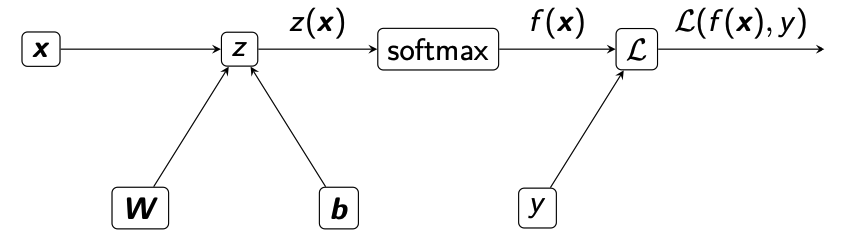
\includegraphics[width=.7\textwidth]{autodiff/computational-graph.png}
    \caption{Computational graph for $\L(\softmax(Wx+b), y)$}
    \label{fig:computational-graph}
\end{figure}
In Figure \ref{fig:computational-graph}, reading from left to right, we can see that the weights $W$, the biases $b$ and the input $x$ are combined to create a function $z(x)$; to the result of this operation is applied $\softmax$, creating $f(x)$. Finally, $f(x)$ is combined with $y$ using the loss function $\L$, giving the final result of the computation, $\L(f(x), y)$.

Computational graphs can then be used to apply the main algorithm to compute the gradient, called \emph{backpropagation}. We will illustrate its behavior by considering the function $f(x, y, z) = (x+y)\times z$, to which is associated the following computational graph:
\begin{figure}[H]
    \centering
    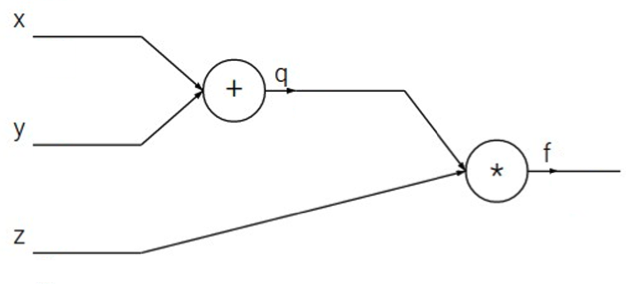
\includegraphics[width=.5\textwidth]{autodiff/simple-graph.png}
    \caption{Computational graph for $f(x, y, z) = (x+y)\times z$}
\end{figure}

\subsubsection{Forward pass}
The first step of backpropagation is to compute the outputs during a \emph{forward pass}. This is simply done by replacing each input by its numerical value, and applying the operations described by the nodes of the graph. Using $x=-2$, $y=5$, $z=-4$ in the previous example yields:
\begin{figure}[H]
    \centering
    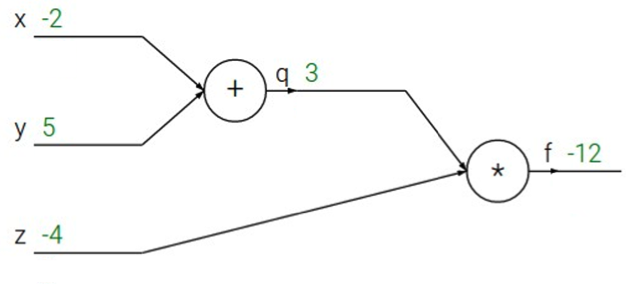
\includegraphics[width=.5\textwidth]{autodiff/forward-graph.png}
    \caption{Forward pass}
\end{figure}

\subsubsection{Backward pass}
The backward pass allows us to compute the derivatives, in our case $\partfrac{f}{x}$, $\partfrac{f}{y}$ and $\partfrac{f}{z}$. Instead of computing the value at each node from left to right (forward pass), we will compute the values of the derivatives from right to left, starting from the output (backward pass).

\begin{itemize}
    \item Starting from the output node, we have that $\partfrac{f}{f}=1$.
    \item Going backward to the $z$ input node, we have that $\partfrac{f}{z}=q$, since $f=qz$. We can then use the results of the forward pass to find the value of $q$, and deduce $\partfrac{f}{z}=3$.
    \item Similarly, $\partfrac{f}{q}=z=-4$.
    \item Going further back into the graph, we aim at computing $\partfrac{f}{y}$. Using chain rule, we know that:
    \begin{equation*}
        \partfrac{f}{y}=\partfrac{q}{y}\partfrac{f}{q}
    \end{equation*}
    This equation can be interpreted in terms of \say{gradient stream}: we want to compute the \emph{downstream gradient} $\partfrac{f}{y}$, that is the gradient \say{after the node}. This gradient can therefore be expressed using the chain rule as the product of the \emph{local gradient} $\partfrac{q}{y}$ and the \emph{upstream gradient} $\partfrac{f}{q}$, that is the gradient computed at the previous node.
    \begin{equation*}
        \underbrace{\partfrac{f}{y}}_{\textnormal{Downstream}}=\underbrace{\partfrac{q}{y}}_{\textnormal{Local}} \underbrace{\partfrac{f}{q}}_{\textnormal{Upstream}}
    \end{equation*}
    Like in previous cases, we can compute the local gradient $\partfrac{q}{y}=1$ since $q=x+y$. The upstream gradient is also known at this point of the pass, due to the backward direction, hence $\partfrac{f}{y}=1\times-4=-4$
    \item The same approach using the chain rule can be used for $\partfrac{f}{x}=\partfrac{q}{x}\partfrac{f}{q}=1\times -4=-4$.
\end{itemize}

\subsubsection{Modularity}
A benefit of backpropagation is its modularity: the gradient computation can be broke down into the computation of the downstream gradient knowing the upstream gradient and the local gradient of the node. 

Consider for instance a function $f$ taking $x$ and $y$ as inputs, and producing an output $z$. This function is a node somewhere in a possibly very complex computational graph, but we do not need the whole information about the rest of the computation: to compute the downstream gradient, we only need local information, that is upstream and local gradients. 

We are given the upstream gradient of the loss that we want to compute with respect to our output, $\partfrac{\L}{z}$. Our goal is now simply to propagate the gradient computation by providing the downstream derivatives, that is $\partfrac{\L}{x}$ and $\partfrac{\L}{y}$. Since we know the expression of $f$, we are able to compute the local derivatives $\partfrac{z}{x}$ and $\partfrac{z}{y}$; using chain rule, we can therefore provide the downstream gradient.
\begin{figure}[H]
    \centering
    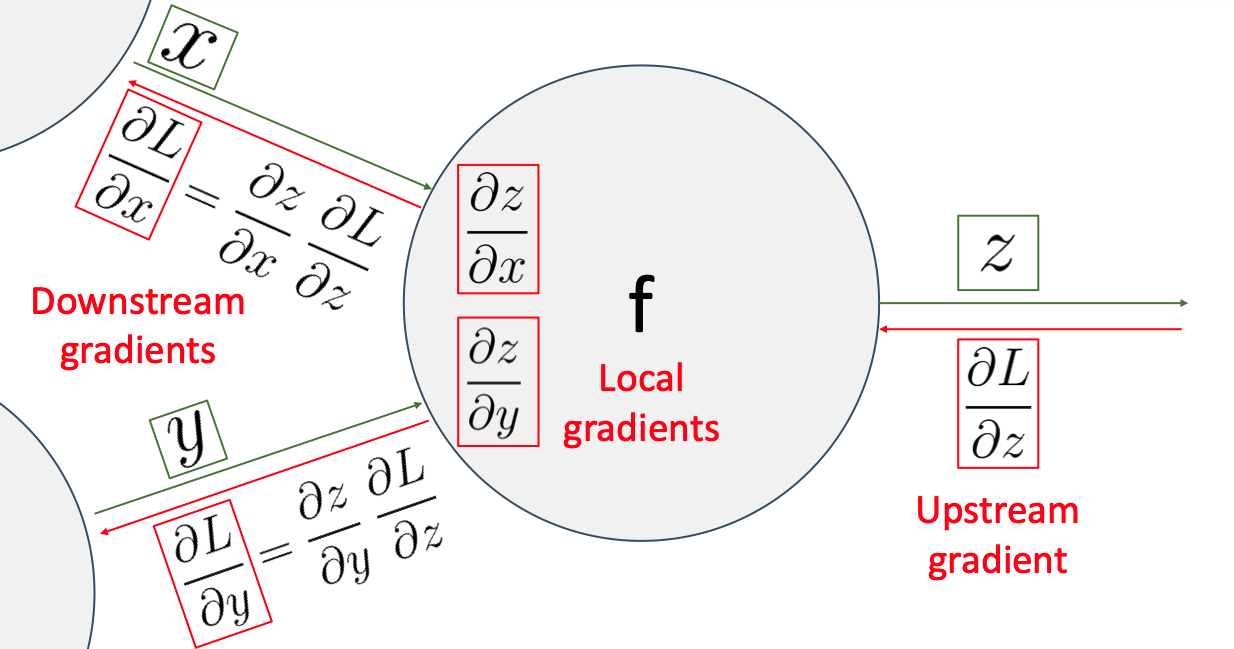
\includegraphics[width=.6\textwidth]{autodiff/modularity.png}
    \caption{Local process of computing the downstream gradient}
\end{figure}

\subsubsection{A complete example}
\begin{figure}[H]
    \centering
    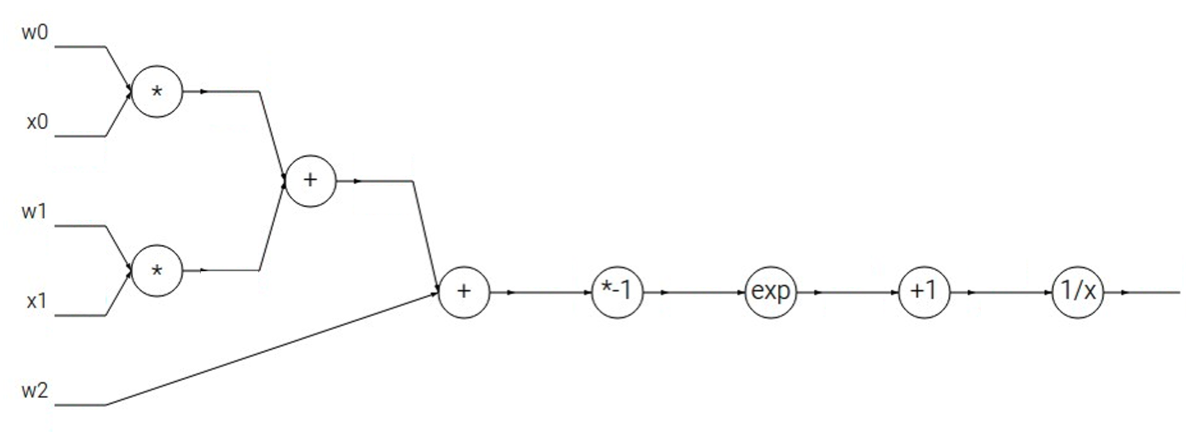
\includegraphics[width=.6\textwidth]{autodiff/complete-example.png}
    \caption{Computational graph for the function $f(x, w) = \frac{1}{1+e^{-(w_0x_0+w_1x_1+w_2)}}$}
\end{figure}
We do not have to break down the gradient computation only into elementary operations such as additions or multiplications: we can define blocks, such as \say{Sigmoid}, and hard-code their gradients to avoid using automatic differentiation on it.

\subsection{Extension to multivariate calculus}
So far, we only considered backpropagation in the case of scalars. The same principle can nevertheless be extended to multivariate calculus using vectors and matrices.

\subsubsection{Reminder on vector derivatives}
For a real-valued function $f:\R\longrightarrow\R$, the regular derivative is a scalar:
\begin{equation*}
    \frac{\dd f}{\dd x} = \partfrac{f}{x} \in \R
\end{equation*}

For a function taking a vector and returning a scalar, that is $f:\R^n\longrightarrow\R$, its derivative is its \emph{gradient}, that is:
\begin{equation*}
    \nabla f\in\R^n \where \left(\nabla f\right)_i = \partfrac{f}{x_i}
\end{equation*}
The $i$-coordinate of the gradient is the partial derivative of $f$ with respect to the $i$-th variable of the input vector.

Finally, for a differentiable function taking a vector and returning another vector, that is $f:\R^n\longrightarrow\R^m$, its derivative is its \emph{Jacobian}, that is:
\begin{equation*}
    J_f 
    = \begin{bmatrix} \partfrac{f}{x_1} & \dots & \partfrac{f}{x_n}\end{bmatrix} 
    = \begin{bmatrix} 
        \nabla^\tp f_1\\ 
        \vdots\\ 
        \nabla^\tp f_m
    \end{bmatrix}
    = \begin{bmatrix}
        \partfrac{f_1}{x_1} & \dots & \partfrac{f_1}{x_n}\\
        \vdots & \ddots & \vdots\\
        \partfrac{f_m}{x_1} & \dots & \partfrac{f_m}{x_n}
    \end{bmatrix}
    \in\mathscr{M}_{m, n}(\R)
\end{equation*}

\subsubsection{Example: linear layer gradient}
Consider a linear layer of the form $f(x)=Wx$ where $W$ is an $m\times n$ matrix. The $i$-th coordinate of the output of is
\begin{equation*}
    f_i = W_ix=\sum_j W_{i,j}x_j
\end{equation*}
where $W_i$ is the $i$-th row of $W$. Therefore, its Jacobian is:
\begin{equation*}
    (J_f)_{i, j} = \partfrac{f_i}{x_j} = W_{i, j}
\end{equation*}
hence $J_f=W$.

\subsubsection{Generalized multivariate chain rule}
Consider two differentiable functions $f:\R^m\longrightarrow\R^k$ and $g:\R^n\longrightarrow\R^m$, and $a\in\R^n$. The chain rule is expressed as:
\begin{equation}
    D_a(f\circ g) = D_{g(a)}f\circ D_ag
\end{equation}
where $D_af$ for instance is the derivative of $f$ evaluated in $a$. Furthermore, the Jacobians verify:
\begin{equation}
    J_{f\circ g}(a)=J_f(g(a)) J_g(a)
\end{equation}

\section{Introduction to Reinforcement Learning}

\section{Optimization and loss functions}

\section{Convolutional Neural Networks}
\subsection{Introduction}
\emph{Convolutional Neural Networks} (CNNs) is a class of models widely used in computer vision. While Fully Connected Neural Networks are very powerful machine learning models, they do not respect the 2D spatial structure of the input images. For instance, training a Multilayer Perceptron on a dataset of $32\times 32$ images required the model to start with a \texttt{Flatten} layer, that reshaped matrix images of size \texttt{(32, 32)} to flattened vectors of size \texttt{(1024, 1)}. Similarly, different color channels were handled separately, reshaping tensor images of dimensions \texttt{(32, 32, 3)} to \texttt{(3072, 1)}.

\begin{figure}[H]
    \centering
    \begin{tikzpicture}
        \newcommand{\randint}{
            \pgfmathsetmacro{\temp}{random(0, 1)}
            \temp
        }
        \fill[orange!60] (-1.9, -1.9) rectangle (1.9, 1.9);
        \matrix [
            matrix of math nodes,
            nodes={
                minimum size=1em, 
                outer sep=0pt,
                inner sep=0,line
                width=0.5pt,
                append after command={
                    \pgfextra{\draw[thick] 
                    ($(\tikzlastnode.north west)+(-0.4em,+0.4em)$)
                    rectangle ($(\tikzlastnode.south east)+(0.4em,-0.4em)$);}
                }
            },
            nodes in empty cells,
            column sep=-0.5pt,
            row sep=-0.5pt
        ]
        {
            \randint & \randint & \randint & \randint & \randint \\
            \randint & \randint & \randint & \randint & \randint \\
            \randint & \randint & \randint & \randint & \randint \\
            \randint & \randint & \randint & \randint & \randint \\
            \randint & \randint & \randint & \randint & \randint \\
        };

        \draw[<->, thick] (-1.9, -2.1) -- (1.9, -2.1) node[below, pos=0.5] {$32$};
        \draw[<->, thick] (-2.1, -1.9) -- (-2.1, 1.9) node[left, pos=0.5] {$32$};

        \draw[-, thick] (2.1, 0) -- (5, 0) node[above, pos=0.5] {Flatten};
        \draw[-, thick] (5, 2) -- (5, -2);

        \draw[->, thick] (5, 2) -- (5.2, 2);
        \draw[->, thick] (5, -2) -- (5.2, -2);

        \foreach \y in {-2, -1.5, ..., 2}
        {
           \node[circle,draw,thick,fill=orange!60] at (5.5, \y) {};
        }

        \draw[<->, thick] (6, 2.1) -- (6, -2.1) node[right, pos=0.5] {$1024$};
    \end{tikzpicture}
    \caption{Flatten layer breaking the spatial strucutre of input data}
\end{figure}

CNNs introduce new operators taking advantage of the spatial structure of the input data, while remaining compatible with automatic differentiation. While MLPs build the basic blocks of Deep Neural Networks using Fully-Connected Layers and Activation Layers, this chapter will introduce three new types of layers: \emph{Convolution Layers}, \emph{Pooling Layers}, and \emph{Normalization}.

\subsection{Convolution Layers}
Similarly to Fully-Connected Layers, \emph{Convolution Layers} have learnable weights, but also have the particularity to respect the spatial information.

\subsubsection{Input shape}
A Fully-Connected layer (also known as Linear layer) receives some flattened vector and outputs another vector:
\begin{figure}[H]
    \centering
    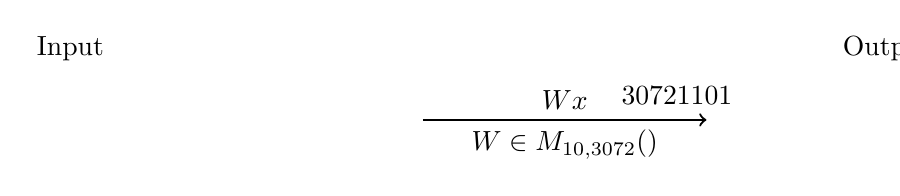
\begin{tikzpicture}
        \node at (-7, 0.7) {Input};
        \parallelepiped{(-4, 0, 0)}{6}{.5}{.5}{$3072$}{$1$}{}{blue!20}

        \draw[->, thick] (-3.4, -.2) -- (0.2, -.2) node[above, pos=.5] {$Wx$} node[below, pos=.5] {$W\in\mathscr{M}_{10,3072}(\R)$};

        \node at (2.5, .7) {Output};
        \parallelepiped{(4, 0, 0)}{3}{.5}{.5}{$10$}{$1$}{}{red!30}
    \end{tikzpicture}
    \caption{Fully-Connected Layer}
\end{figure}

Instead, a CNN takes as an input a 3D volume: for instance, an image can be represented as a tensor of shape $3\times32\times32$, the first dimension being the number of channels (red, green, blue), and the other two being the width and height of the image.

\subsubsection{Kernels}
The convolutional layer itself consists of small kernels (also called filters) used to \emph{convolve} with the image, that is sliding over it spatially, and computing the dot products at each possible location.
\begin{definition}[Kernel]
    A \emph{kernel} (or \emph{filter}) is a tensor of dimensions $D\times K\times K$, where $D$ is the number of channels (or \say{depth}) of the input, and $K$ is a parameter called \emph{kernel size}.
\end{definition}

\begin{definition}[Convolution of two matrices]
    Given two matrices $A=(a_{i, j})_{i, j}$ and $B=(b_{i, j})_{i, j}$ in $\mathscr{M}_{m, n}(\R)$, the \emph{convolution of $A$ and $B$}, noted $A*B\in\R$, is the following:
    \begin{equation}
        A*B = \sum_{i=1}^m \sum_{j=1}^n a_{(m-i+1), (n-j+1)} \cdot b_{i, j}
    \end{equation}
    This corresponds to the dot product in the space $\mathscr{M}_{m, n}(\R)$.
\end{definition}

\begin{definition}[Kernel convolution]
    An input of shape $C\times H\times W$ can be processed by a kernel of shape $C\times K\times K$ by computing at each possible spatial position the convolution between the kernel and the submatrix of the input. 
    \begin{figure}[H]
        \centering
        \begin{tikzpicture}[scale=.5]
            \tdplotsetmaincoords{70}{140}
            \begin{scope}[tdplot_main_coords,canvas is yz plane at x=0]
                \draw[fill=orange!50, thick] (0,0) rectangle (3, 3);
                \draw (0,0) grid (3, 3);

                \draw[fill=blue!30, thick] (9, 4) rectangle (12, 7);
                \draw (8,0) grid (16, 8);

                \draw[thick,dotted] (0, 0) -- (9, 4);
                \draw[thick,dotted] (0, 3) -- (9, 7);
                \draw[thick,dotted] (3, 0) -- (12, 4);
                \draw[thick,dotted] (3, 3) -- (12, 7);

                \draw[fill=red!50, thick] (19, 8) rectangle (20, 9);
                \draw (18,4) grid (24, 10);

                \draw[thick,dotted] (9,4) -- (19,8);
                \draw[thick,dotted] (9,7) -- (19,9);
                \draw[thick,dotted] (12,4) -- (20,8);
                \draw[thick,dotted] (12,7) -- (20,9);

                \node at (1.5, -1.5) {Kernel};
                \node at (11.5, -1.5) {Input};
                \node at (22, 2.5) {Activation map};
            \end{scope}
        \end{tikzpicture}
        \caption{Kernel convolution}
    \end{figure}
    
    The output of this operation in an \emph{activation map} of dimension $1\times (H - K + 1) \times (W - K + 1)$ representing for each pixel the convolution between the kernel and the corresponding chunk of the image.
    \begin{figure}[H]
        \centering
        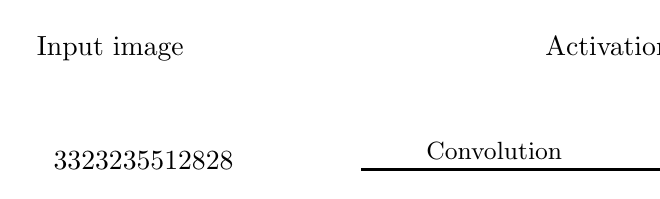
\begin{tikzpicture}[scale=.9]
            \node at (.8, 1.7) {Input image};
            \parallelepiped{(0, 0, 0)}{.5}{4}{3}{$3$}{$32$}{$32$}{blue!20}
            \parallelepiped{(1.3, .3, .3)}{.5}{1.2}{.9}{$3$}{$5$}{$5$}{orange!50}

            \node at (6.7, 1.7) {Activation map};
            \parallelepiped{(6, 0, 0)}{.2}{3.8}{2.8}{$1$}{$28$}{$28$}{red!30}
            \draw[->, thick] (1.8, 0) -- (6.5, 0) node[above, pos=.4] {\small Convolution};

            \parallelepiped{(7.45, .85, 2)}{.15}{.25}{.2}{}{}{}{orange!50}
        \end{tikzpicture}
        \caption{Input and output of the convolution operation}
        \label{fig:one-kernel-layer}
    \end{figure}
\end{definition}

Intuitively, the result of the kernel convolution tells us for each pixel \emph{how much the neighbourhood of the input pixel corresponds to the kernel}.

\begin{example}[Gaussian blur]
    Let $G\in\mathscr{M}_{3}(\R)$ be the following kernel:
    \begin{equation*}
        G := \frac{1}{16}\begin{bmatrix}
            1 & 2 & 1\\
            2 & 4 & 2\\
            1 & 2 & 1
        \end{bmatrix}
    \end{equation*}
    Each coefficient of this matrix is an approximation of the Gaussian distribution. Applying this kernel to an image produces a smoothed version of the input.
\end{example}
% TODO: add gaussian blur image

\begin{example}[Sobel operator]
    Let $S_x$ and $S_y\in\mathscr{M}_{3}(\R)$ be the following kernels:
    \begin{equation*}
        S_x := \begin{bmatrix}
            +1 & 0 & -1\\
            +2 & 0 & -2\\
            +1 & 0 & -1
        \end{bmatrix}
        \qquad\textnormal{and}\qquad
        S_y := S_x^\tp = \begin{bmatrix}
            +1 & +2 & +1\\
            \phantom{+}0 & \phantom{+}0 & \phantom{+}0\\
            -1 & -2 & -1
        \end{bmatrix}
    \end{equation*}
    The convolution between these operators and an image produces horizontal and vertical derivatives approximations of the image pixels.

    \begin{figure}[H]
        \centering
    
        \begin{minipage}{0.4\textwidth}
            \centering
            \caption*{Input image}
            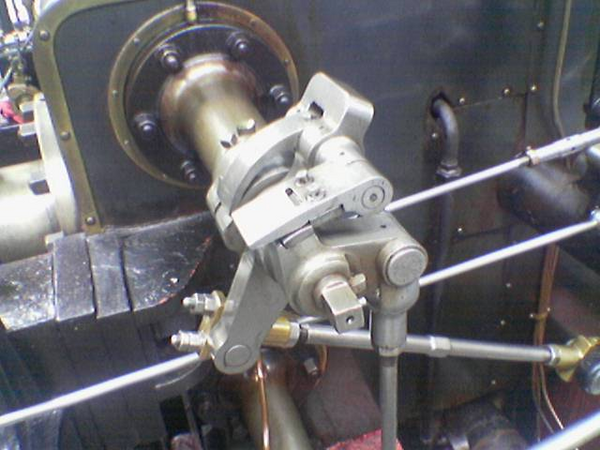
\includegraphics[width=.9\textwidth]{images/pre-sobel.png}
        \end{minipage}
        \begin{minipage}{0.4\textwidth}
            \centering
            \caption*{Sobel operator applied to the image}
            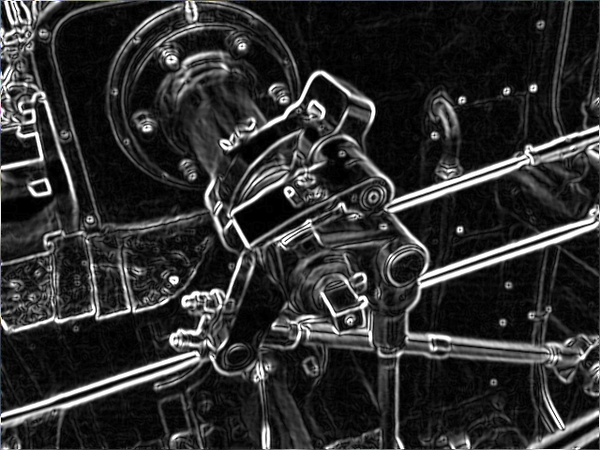
\includegraphics[width=.9\textwidth]{images/post-sobel.png}
        \end{minipage}
        
        \caption{Effect of the Sobel operator on an image}
    \end{figure}
\end{example}

These two examples show that kernels used in convolutional layers express meaningful transformations of the input, justifying their use in CNNs. For instance, one could hardcode different kernels (gaussian blur, Sobel operator, vertical/horizontal lines extraction) to extract interesting features from an image, and plug these features into an MLP to obtain an improved classifier compared to a basic, flattening MLP. We will see that instead, CNNs have learnable kernel weights, allowing the model to choose the kernels that it considers bests.

\subsubsection{Multiple kernels}
In Figure \ref{fig:one-kernel-layer}, we used simply one kernel to compute one activation map. In practice, we repeat this process multiple times: we consider a set (or \emph{bank}) of filters having different weights values, and for each kernel of the set, we compute its activation map.
\begin{figure}[H]
    \centering
    \begin{tikzpicture}
        % Input
        \node at (.8, 1.7) {Input image};
        \parallelepiped{(0, 0, 0)}{.5}{4}{3}{$3$}{$32$}{$32$}{blue!20}

        % Convolution Layer
        \draw[thick] (1.5, -1) -- ++ (2.25, 0);
        \node[rectangle,draw,thick,rounded corners] at (5, -1) {\begin{varwidth}{2.5cm}\centering Convolution Layer\end{varwidth}};
        \draw[thick, ->] (6.25, -1) -- ++ (2.25, 0);

        % Kernels
        \node at (5, -4.5) {6 kernels};
        \draw[thick, ->] (5.1, -2.5) -- ++ (0, 0.9);
        \parallelepiped{(3.8, -3, 0)}{.3}{1}{.75}{$3$}{$5$}{}{orange!40};
        \foreach \x in {4.3, 4.8, ..., 5.8} {
            \parallelepiped{(\x, -3, 0)}{.3}{1}{.75}{}{}{}{orange!40};
        }
        \parallelepiped{(6.3, -3, 0)}{.3}{1}{.75}{}{}{$5$}{orange!40};

        % Activation maps
        \node at (10.8, 1.7) {6 activation maps};
        \parallelepiped{(9, 0, 0)}{.2}{3.5}{2.75}{$1$}{$28$}{}{red!40};
        \foreach \x in {9.5, 10, ..., 11} {
            \parallelepiped{(\x, 0, 0)}{.2}{3.5}{2.75}{}{}{}{red!40};
        }
        \parallelepiped{(11.5, 0, 0)}{.2}{3.5}{2.75}{}{}{$28$}{red!40};
        \node at (10.7, -4.5) {$6\times28\times28$ output};
    \end{tikzpicture}
    \caption{Convolutional Layer using 6 kernels}
\end{figure}

Using a bank containing $C'$ filters, the output of the convolutional layer in an \emph{activation map} of dimension $C'\times (H - K + 1) \times (W - K + 1)$ representing for each pixel the convolution between the given kernel and the corresponding chunk of the image.

\begin{remark}[Biases in Convolutional Layers]
    Similarly to fully-connected layers, we often add to the activation map of each kernel a bias of size $1\times (H - K + 1) \times (W - K + 1)$. Those biases might me ommited in the rest of the chapter for the sake of simplicity.
\end{remark}

\subsubsection{Stacking convolutions}
Like previously introduced layers, convolutional layers can be stacked to form deep networks. The layer shapes need to match, in particular the output channels of a layer must match the input channels of the next layer, and the output height and width must match the next input height and width.
\begin{figure}[H]
    \centering
    \begin{tikzpicture}
        % Input
        \node at (.5, 1.9) {\begin{varwidth}{3cm}\centering Input image $3\times32\times32$\end{varwidth}};
        \parallelepiped{(0, 0, 0)}{.5}{4}{3}{$3$}{$32$}{$32$}{blue!20}

        % Convolution layer
        \draw[thick] (1.5, -1) -- ++ (.8, 0);
        \node[rectangle,draw,thick,rounded corners] at (3, -1) {Conv.};
        \draw[thick, ->] (3.7, -1) -- ++ (.8, 0);
        \node at (3, -.3) {$6\times3\times5\times5$};

        % First hidden layer
        \node at (6, 1.7) {\begin{varwidth}{3.5cm}\centering First hidden layer $3\times28\times28$\end{varwidth}};
        \parallelepiped{(5.75, 0, 0)}{1}{3.5}{2.5}{$6$}{$28$}{$28$}{red!40}

        % Convolution layer
        \draw[thick] (7, -1) -- ++ (.8, 0);
        \node[rectangle,draw,thick,rounded corners] at (8.5, -1) {Conv.};
        \draw[thick, ->] (9.2, -1) -- ++ (.8, 0);
        \node at (8.5, -.3) {$10\times6\times3\times3$};

        % Second hidden layer
        \node at (11.5, 1.5) {\begin{varwidth}{4cm}\centering Second hidden layer $3\times26\times26$\end{varwidth}};
        \parallelepiped{(11.5, 0, 0)}{1.3}{3.1}{2.1}{$10$}{$26$}{$26$}{green!20}

        % Convolution layer
        \draw[thick] (12.5, -1) -- ++ (.8, 0);
        \node[rectangle,draw,thick,rounded corners] at (14, -1) {Conv.};
        \draw[thick, ->] (14.7, -1) -- ++ (.8, 0);
        \node at (14, -.3) {$12\times10\times3\times3$};
    \end{tikzpicture}
    \caption{Stacking of 3 Convolutional Layers of correct shapes}
\end{figure}

However, stacking two convolution layers next to each other produces another convolutional layers, and do not add representation power. Therefore, we use the exact same solution as for linear classifiers: we introduce non-linear layers using activation functions in between convolutional layers.
\begin{figure}[H]
    \centering
    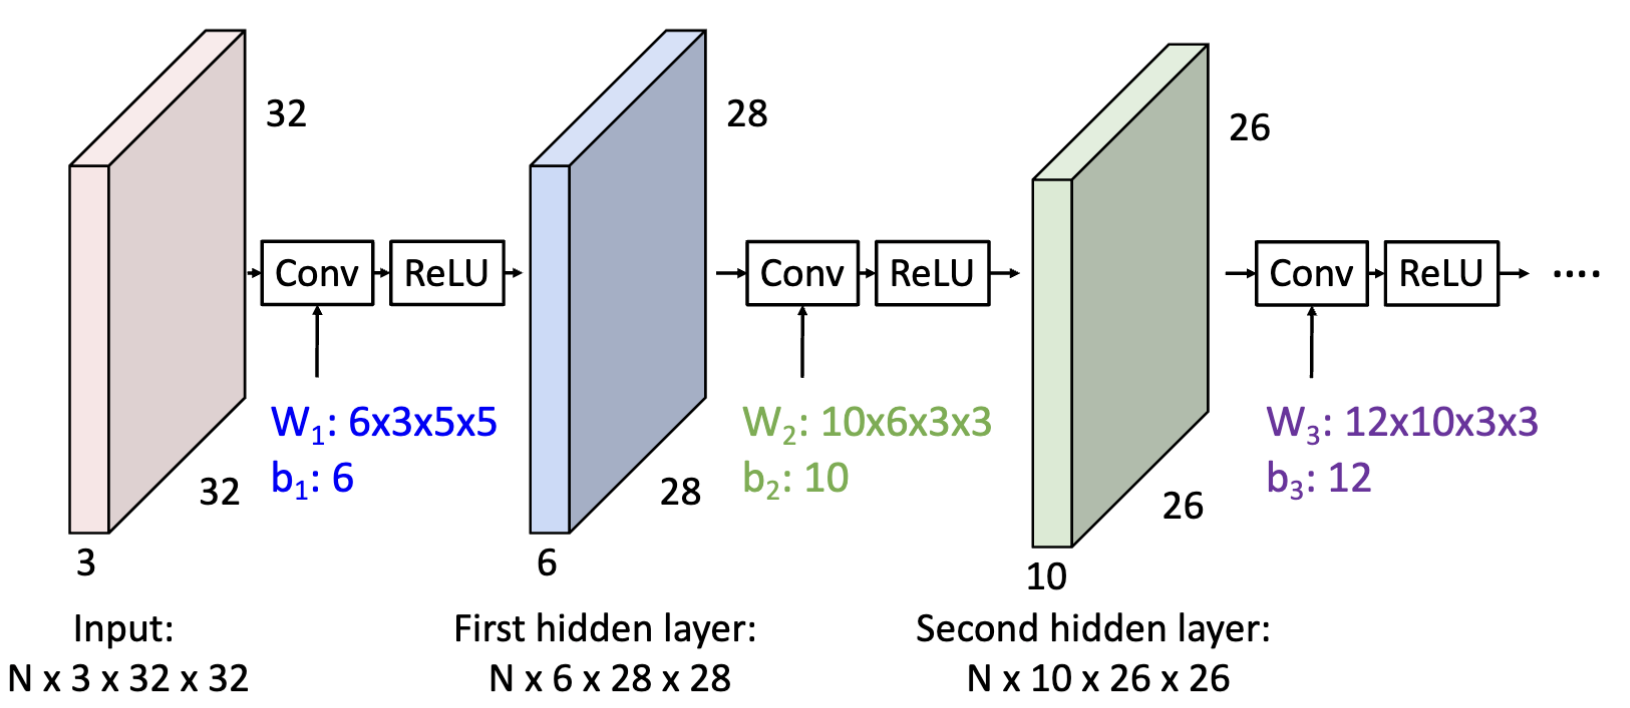
\includegraphics[width=0.7\textwidth]{images/stacking-conv-relu.png}
    \caption{Adding ReLU layers in between Convolution Layers}
\end{figure}

\subsubsection{Spatial dimensions and Padding}
As stated previously, using an input of width $W$ with a filter of kernel size $K$, the output width is $W-K+1$. A problem with the approach is that features maps decrease in size with each layer. This creates an upper bound on the maximum number of layers that we can use for our model. 

A solution to this is to introduce \emph{padding} by adding zeros around the border of the input. When the kernel will slide around the edges of the input, a part of the coefficients that it will consider in its convolution will be zeros.
\begin{figure}[H]
    \centering
    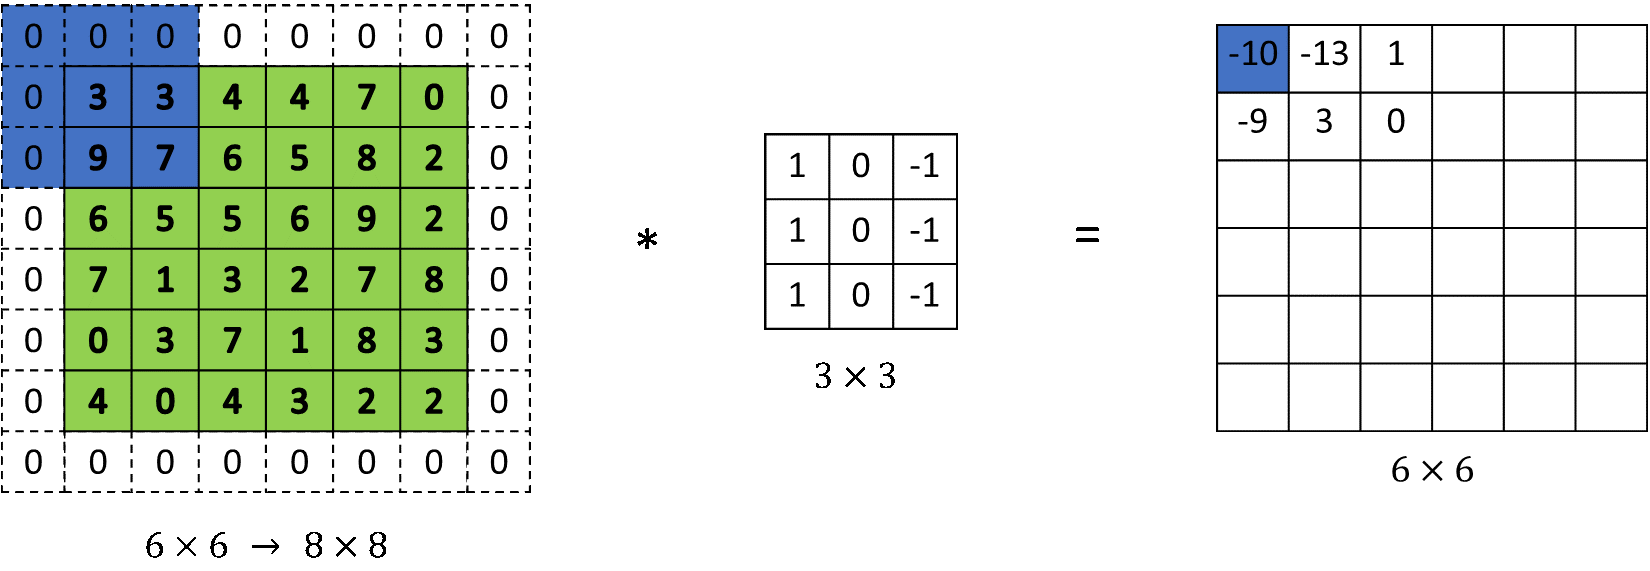
\includegraphics[width=0.7\textwidth]{images/padding.png}
    \caption{Adding padding around the input}
\end{figure}

\begin{remark}[Padding strategies]
    Even though we might imagine different padding strategies instead of always padding with zeros (for instance, nearest-neightbour padding, circular padding, random padding\dots), zero-padding seems to be both simple and effective in practice, and is the most commonly used strategy.
\end{remark}

Padding introduces an additional hyperparameter to the layer, $P$. 
Using padding, the width of the output of the layer becomes:
\begin{equation}
    \label{eq:output-padding}
    W'=W-K+2P+1
\end{equation}
A common way to set the value of $P$ is to choose it such as the output have the same size as the input. This is achieved by taking $P=(K-1)/2$, called \emph{same-padding}.

\subsubsection{Receptive Fields}
\begin{definition}[Receptive Field]
    The \emph{receptive field} of an output neuron is the set of neurons of the input of which the output neuron depends on.
\end{definition}

By essence, Fully-connected layers have a trivial notion of receptive field: an output neuron is connected to each input neuron, its receptive field is therefore the entire input.

Convolution layers are build in such a way that each element in the output simply depends on a receptive field of size $K$ (that is a square of area $K\times K$) in the input. As we stack convolutional layers after the others, each successive convolution adds $K-1$ to the receptive field size. After $L$ layers, the receptive field size is $1+L\times(K-1)$. 

\begin{figure}[H]
    \centering
    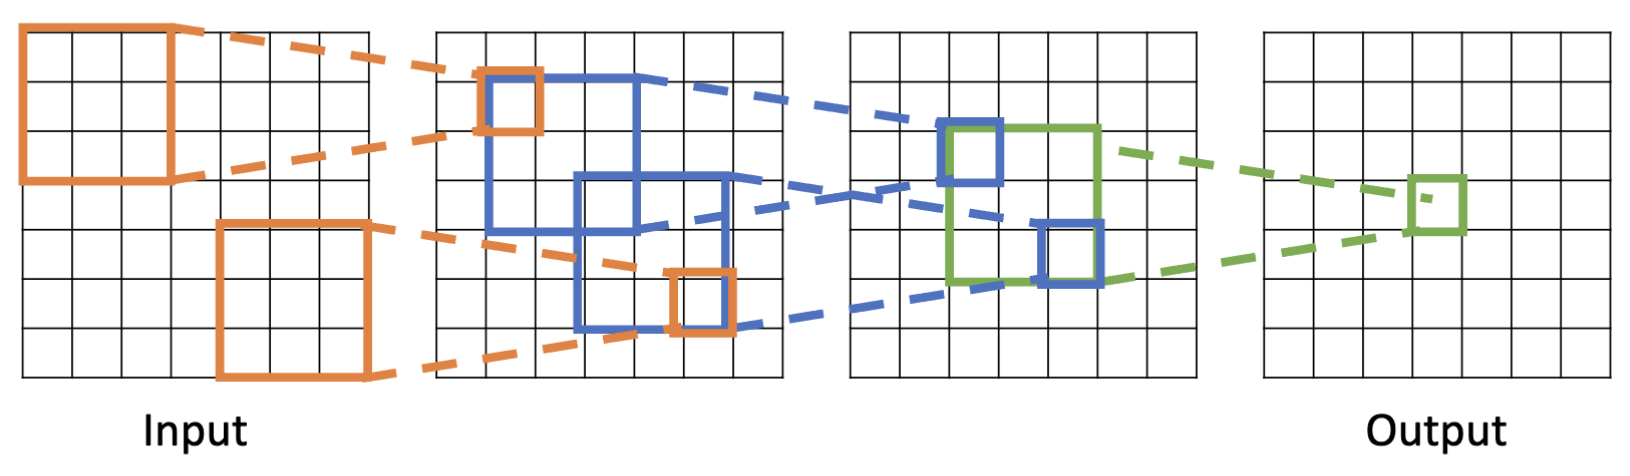
\includegraphics[width=0.8\textwidth]{images/receptive-field.png}
    \caption{Receptive field of an output neuron}
\end{figure}

This linear growth shows that by stacking enough layers, each output neuron will eventually have the entire input image in its receptive field. Nevertheless, this can be a problem in practice as we might need many layers for each output to depend on the whole image.

A solution to this problem is to downsample the image size inside the network. This can be done by adding another hyperparameter, \emph{stride}.

\subsubsection{Strided Convolution}
\begin{definition}[Stride]
    The hyperparameter \emph{stride} defines the number of pixels between two applications of the kernel.
\end{definition}
\begin{wrapfigure}{r}{0.4\textwidth}
    \centering
    \begin{tikzpicture}
        \newcommand{\randint}{
            \pgfmathsetmacro{\temp}{random(0, 1)}
            \temp
        }
        \fill[orange!60] (-2, -2) rectangle (2, 2);
        \matrix [
            matrix of math nodes,
            nodes={
                minimum size=1em, 
                outer sep=0pt,
                inner sep=0,line
                width=0.5pt,
                append after command={
                    \pgfextra{\draw[thick] 
                    ($(\tikzlastnode.north west)+(-0.3em,+0.3em)$)
                    rectangle ($(\tikzlastnode.south east)+(0.3em,-0.3em)$);}
                }
            },
            nodes in empty cells,
            column sep=-0.5pt,
            row sep=-0.5pt
        ]
        {
            \randint & \randint & \randint & \randint & \randint & \randint \\
            \randint & \randint & \randint & \randint & \randint & \randint \\
            \randint & \randint & \randint & \randint & \randint & \randint \\
            \randint & \randint & \randint & \randint & \randint & \randint \\
            \randint & \randint & \randint & \randint & \randint & \randint \\
            \randint & \randint & \randint & \randint & \randint & \randint \\
        };

        \draw[densely dashed, color=red, line width=1mm] (-2, 0) rectangle (0, 2);
        \draw[color=red, line width=1mm] (-2/3, 0) rectangle (4/3, 2);

        \draw[<->, color=red, thick] (-2, 2.2) -- (-2/3, 2.2) node[above, pos=.5] {stride};
    \end{tikzpicture}
    \caption{Effect of stride}
\end{wrapfigure}

Stride effectively downsamples the size of the image. Applying a convolution between an image of width $W$ and padding $P$ with a kernel of size $K$ and stride $S$ produces the following output dimension:
\begin{equation}
    \label{eq:output-stride}
    W'=\frac{W-K+2P}{S}+1
\end{equation}
Note that choosing $S=1$ in \eqref{eq:output-stride} gives the same result as \eqref{eq:output-padding}. Depending on the implementation, the result can be rounded up or down in the case where it is not an integer. Usually, all the parameters are chosen such that $S$ divides $W-K+2P$.

\subsection{Pooling Layers}
\subsubsection{Introduction}
Computer Vision, one of the most frequent use for CNNs, often deals with images of high quality, making downsampling an important task to drastically reduce the number of layers and the quantity of VRAM used by the model. We saw a first approach to downsampling embedded in Convolutional Layers, that is strided convolution. Pooling Layers are layers dedicated to downsampling, without learnable parameters.

Pooling layers work similarly to convolutional layers, using a mechanism of kernels. Nevertheless, instead of applying a convolution between some kernel and the image, the layer will apply a pooling function to the area of the input. This will produce an activation map with dimensions depending on the hyperparameters of the layer -- kernel size, padding and stride, the same as the parameters of a convolutional layer.

\begin{figure}[H]
    \centering
    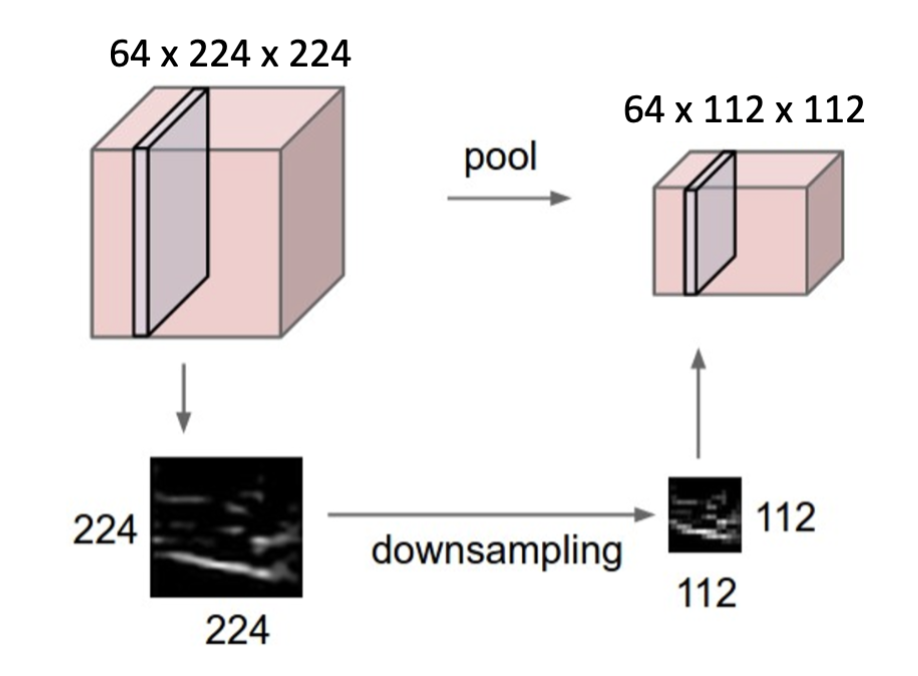
\includegraphics[width=0.5\textwidth]{images/pooling-layer.png}
    \caption{Behavior of a pooling layer}
\end{figure}
Another difference is that the operation is applied for each slice of the input volume. Choosing appropriate values for the hyperparameters (for instance $S\geq2$, \dots) allow to downsample the input without the need for learnable parameters.

\subsubsection{Max Pooling}
\begin{definition}[Max Pooling function]
    For $K\geq 1$, the \emph{Max Pooling function} of kernel size $K$ is:
    \begin{equation*}
        \begin{aligned}
            \textnormal{max}_P: \mathscr{M}_{K}(\R) &\longrightarrow \R\\
            (m_{i, j}) &\longmapsto \max_{i, j} m_{i, j}
        \end{aligned}
    \end{equation*}
\end{definition}

A \emph{Max Pooling} layer applies the Max Pooling function to each location of size $K\times K$ in each slice of the input volume. We often choose the same kernel size as the slide (that is $K=S$) to avoid recovering twice the same pixel value. In this setting, it is equivalent to spliting each input channel into non-overlapping regions of size $K\times K$, from which are extracted the maximum value of the section and stored in the output channel.

Max Pooling has some advantages over convolutional layers with stride: it does not involve learnable parameters, reducing the computational cost, but also introduces translational invariance to small spatial shifts. Indeed, if the position of a specific maximum pixel is moved slightly, we might intuitively think that it will stay the maximum of its region, making the model robust to small translations.

\subsubsection{Average Pooling}
\begin{definition}[Average Pooling function]
    For $K\geq 1$, the \emph{Average Pooling function} of kernel size $K$ is:
    \begin{equation*}
        \begin{aligned}
            \textnormal{avg}_P: \mathscr{M}_{K}(\R) &\longrightarrow \R\\
            (m_{i, j}) &\longmapsto \frac{1}{K^2}\sum_{i=1}^K \sum_{j=1}^K m_{i, j}
        \end{aligned}
    \end{equation*}
    It simply returns the average of the matrix coefficients.
\end{definition}

Average Pooling works exactly the same as Max Pooling, but applying $\textnormal{avg}_P$ as a pooling function instead of $\textnormal{max}_P$.

\subsection{A full CNN example: LeNet-5}
Now that we have these different types of layers, we can stack them together to create a full CNN architecture. A classic model often fits the following architecture:
\begin{equation*}
    (\texttt{Conv, ReLU, Pooling})^{N_1} \rightarrow \texttt{Flatten} \rightarrow (\texttt{Linear, ReLU})^{N_2} \rightarrow \texttt{Linear}
\end{equation*}

As an example, we will take the 1998 model \emph{LeNet-5}:
\begin{figure}[H]
    \centering
    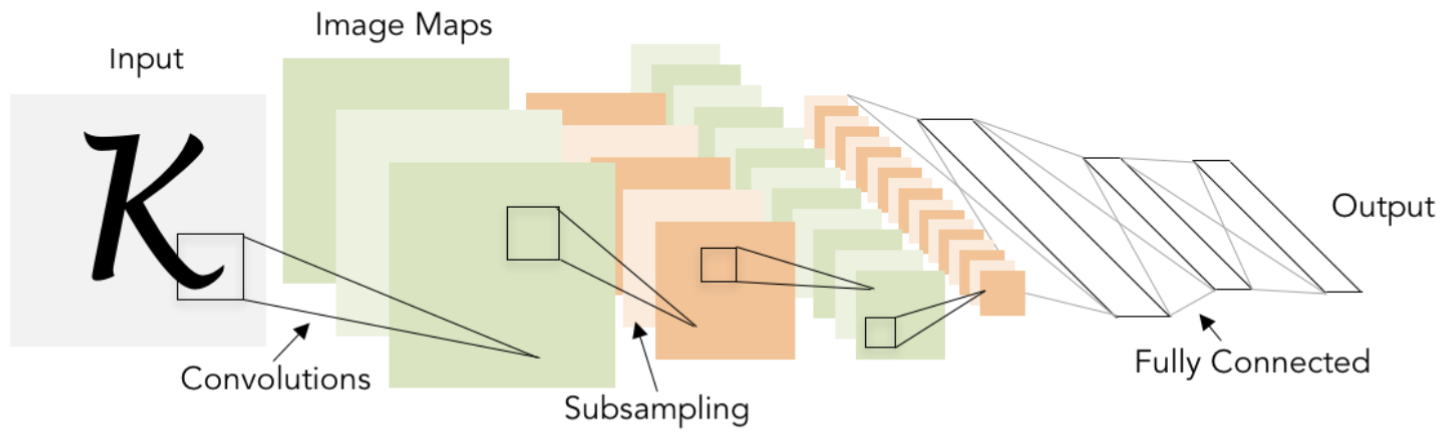
\includegraphics[width=0.8\textwidth]{images/lenet-5.png}
    \caption{LeNet-5 architecture}
\end{figure}
The first blocks of Convolutional and Pooling layers progressively decrease the spatial size of the input, while increasing the number of channels: the total volume of the input is preserved.

\subsection{Normalization}
Deep convolutional neural networks are described previously can be extremly effective when trained; nevertheless, they are also very difficult to train, and we need to properly prepare data for the descent to converge.

A recent solution to ease the training is to add \emph{normalization layers} in the network.

\section{Recursive Neural Networks}

\section{Attention and Transformers}

\section{Robustness and regularity}

\section{Q-Deep Learning for Breakout}

\section{Autoencoders}

\section{Generative Adversarial Networks}

\section{Normalizing Flows}

\end{document}